%% Documentclass:
%% Network Neuroscience
%\documentclass[finalfonts,NETN]{stjour}
\documentclass[NETN]{stjour}
\usepackage{comment}

%% or 

%% Manuscript, for double spaced, larger fonts
%\documentclass[manuscript]{stjour}
%% Only needed if you use `manuscript' option
% \journalname{Network Neuroscience}

%%%%%%%%%%% Article Set-Up %%%%%%%%%%%%%%%%%%%%%%%%%%%%%%%%%%%%
%% Article Type:
%% Default is Research.

%% Or, choose one of these options:
%% Research, Methods, Data, Review, and Perspective

\articletype{Research Article}

%%%%%%%%%%% Please supply information %%%%%%%%%%%%%%%%%%%%%%%%%

\supportinginfo{dx.doi.org/10.7910/DVN/PQ6ILM}

%% if no conflicts, this command doesn't need to be used
%% \conflictsofinterest{}

%%%%%%%%%%% to be supplied by MIT Press, only %%%%%%%%%%%%%%%%%
\citation{Betzel, R. F., Fukushima, M.,w
He, Ye,
Zuo, Xi-Nian,
Sporns, O. (2016)\\
Dynamic fluctuations coincide with periods of high and low modularity
in resting-state functional brain  networks\\
Network Neuroscience, 1
}

\received{20 October 2016}
\accepted{7 November 2016}
\published{26 January 2016}
\setdoi{10.1162/NETN-00001} %% ???

\handlingeditor{Xi-Nian Zuo}

%%%%%%%% End MIT Press commands %%%%%%%%%%

%%%%%%%%%%%%%%%%%%%%%%%%%%%%%%%%%%%%%%%%%%%%%%%%%%%%%%%%%%%%%%%
%% author definitions should be placed here:

%% example definition
\def\taupav{\tau_{\mathrm{Pav}}}

\begin{document}
\title[Co-citations in context]{Co-citations in context}
\subtitle{disciplinary heterogeneity is relevant}

%% If shortened title for running head is needed so that the article title can fit
%%   in the running head, use [] argument, ie,
%%
%%   \title[Shortened Title for Running Head]{Title of Article}
%%   \subtitle{Subtitle Here}

%% Since we use \affil{} in the argument of the \author command, we
%% need to supply another version of the author names, without \affil{}
%% to be used for running heads:

\author[Author Names]
{James Bradley\affil{1},
Sitaram Devarakonda\affil{2}, Avon Davey\affil{2}, Dmitriy Korobskiy\affil{2}, Siyu Liu\affil{2}, Djamil Lakhdar-Hamina\affil{2},Tandy Warnow\affil{3}
\and George Chacko\affil{2}}

\affiliation{1}{Raymond A. Mason School of Business, College of William and Mary, Williamsburg, VA, USA}
\affiliation{2}{Netelabs, NET ESolutions Corporation, McLean, VA 22102, USA}
\affiliation{3}{Department of Computer Science, University of Illinois at Urbana-Champaign, Champaign, IL 61820, USA}


%ie.
%\affiliation{1}{Gatsby Computational Neuroscience Unit, University
%College London, London, United Kingdom} 

%\affiliation{2}{Another Department, Institution, City, Country}

%ie
%\affiliation{2}{Center for Studies in
%Behavioral Neurobiology, Concordia University, Montreal, Quebec,
%Canada}

\correspondingauthor{George Chacko}{netelabs@nete.com}

% ie,
\correspondingauthor{George Chacko}{netelabs@nete.com}

\keywords{co-citation analysis, bibliometrics, random graphs }

%ie
%\keywords{work, leisure, normative, microscopic,  reinforcement learning, economics}

\begin{abstract}
Citation analysis of the scientific literature has been used to study and define disciplinary boundaries, to trace the dissemination of knowledge, and to estimate impact. Co-citation, the frequency with which pairs of publications are cited, provides insight into how documents relate to each other and across fields. Co-citation analysis has been used to characterize combinations of prior work as conventional or innovative and to derive features of highly cited publications. Given the organization of science into disciplines, a key question is the sensitivity of such analyses to frame of reference. Our study examines this question using  semantically-themed citation networks. We observe that trends reported to be true across the scientific literature do not hold for focused citation networks, and we conclude that co-citation analysis requires a contextual perspective.
\end{abstract}

% \begin{authorsummary} 
% \end{authorsummary}
\section{Introduction}

Citation and network analysis of  scientific literature reveals information on semantic relationships between publications, collaboration between scientists, and the practice of citation itself~\citep{garfield_citation_1955,de_solla_price_networks_1965,newman_structure_2001,Shi:2010:CHI:1816123.1816131,patience_pmid28560354}. Co-citation, the frequency with which two documents are cited together in other documents provides additional insights, including the identification of semantically related documents, fields, specializations, and new ideas in science~\citep{small_co-citation_1973, marshakova-shaikevich_co-citation_1973,boyack_co-citation_2010, 10.3389/frma.2018.00020}. 

\cite{uzzi_atypical_2013} used a novel approach for co-citation analysis to characterize a subset of highly cited articles with respect to both novel and conventional combinations of prior research. The frequency with which references were co-cited  in 17.9 million articles and their cited references from the Web of Science (WoS) was calculated and expressed as journal pair frequencies (observed co-citation frequencies). Expected co-citation values were generated from randomized networks using Monte Carlo simulations under a random graph model. Observed frequencies were then normalized (shifted and scaled) to averaged expected values from ten randomized networks and termed as \emph{z-scores}. Consequently, every article was associated with multiple z-scores corresponding to co-cited journal pairs in its references. For each article, positional statistics of z-scores were calculated and evaluated to set thresholds for a binary classification of conventionality using the median z-score of an article and novelty using the tenth percentile of z-scores within an article.

Thus, HCLN would denote high conventionality (HC) and low novelty (LN), with all four combinations of LC and HC with LN and HN being possible. The authors observed that HCHN articles were twice as likely to be highly cited compared to the background rate, suggesting that novel combinations of ideas flavoring a body of conventional thought were a feature of impact. 

Key to Uzzi {\em et al.}, is their random graph model and its underlying assumptions. The citation switching algorithm used to generate expected values by random substitutions of references is designed to preserve the number of publications, the number of references in each publication, and the year of publication of both publications and references. Importantly, disciplinary origin does not affect the probability that a reference is selected to replace another one. For example, a reference in quantum physics can be substituted, with equal probability, by a reference in quantum physics, quantum chemistry, classical literature, entomology, or anthropology. Such substitutions poorly model the disciplinary nature of scientific endeavor and citation behavior~\citep{wallace_lariviere_gingras_2012,moed_measuring_2010,klavans_research_2017,garfield_1979}. In addition, under this random model, a reference cited many times in a given year is selected with the same probability as a reference cited only once, which appears inconsistent with the power law or lognormal citation distributions described in the literature~\citep{stringer_statistical_2010,perline_strong_2005}.  Accordingly, model misspecification is likely to arise on account of the simulated values not reflecting the empirical data very well. 

A follow-up study by \cite{boyack_vs_uzzi_2014} explored the impact of discipline and journal effects on these definitions of conventionality and novelty.  While their study had some methodological differences in the use of Scopus data rather than WoS data, a smaller dataset, and a $\chi^2$ calculation rather than Monte Carlo simulations to generate expected values of journal pairs, Boyack and Klavans noted strong effects from both disciplines and journals. While they also reported the trend that HCHN is more probable in highly cited papers, they observed that ``only 64.4\%  of  243  WoS  subject  categories'' in the Uzzi {\em et al.} study met the criterion of having the highest probability of hit papers in the HCHN category.  Further, they observed that journals vary widely in terms of size and influence and that 20 journals accounted for nearly 15\% of co-citations in their measurements. Lastly, they noted that three multidisciplinary journals accounted for 9.4\% of all atypical combinations. 

Despite different methods used to generate expected values, both of these key preceding studies measured co-citation frequencies across the scientific literature (using either WoS or Scopus) and normalized them without disciplinary constraints before subsequently analyzing disciplinary subsets. We hypothesized instead that modifying the normalization to constrain substitution references to be drawn only from the citation network being studied (the ``local network") rather than all of WoS
(the ``global network") would reduce model misspecification by limiting substitutions from disciplinarily ectopic references. Consequently, we used keyword searches of the scientific literature to construct exemplar citation networks themed around academic disciplines of interest: \emph{applied physics, immunology, and metabolism}. Within these disciplinary frameworks, we calculated observed and expected co-citation frequencies using a refined random graph model and an efficient Monte Carlo simulation algorithm.

Our analyses, using multiple techniques, provides substantial evidence that a constrained model where reference substitutions are limited to a local (disciplinary) network reduces model misspecification compared to the unconstrained model that uses the global network (WoS). Furthermore, re-analyses of these three semantically-themed citation networks  under the improved model reveals strikingly different trends. For example, while Uzzi {\em et al.} reported that highly cited articles are more likely than expected to be both HC and HN and that this trend largely held across all disciplines, we find that these trends vary with the discipline and that universal trends are not apparent. Specifically,  HC remains highly correlated with highly cited articles in the immunology and metabolism datasets but not with applied physics, and HN is highly correlated with highly cited articles in applied physics but not with immunology and metabolism.  Thus, disciplinary networks are different from each other, and trends that hold for the full WoS network do not hold for even large networks (such as metabolism).  Furthermore, we also found that the categories HC, HN, etc.,  demonstrating the highest percentage of highly cited articles are not robust with respect to varying thresholds for high citation counts or for highly novel citation patterns. Overall, our study, although limited to three disciplinary networks, suggests that co-citation analysis that inadequately considers disciplinary differences, may not be very useful at detecting universal features of impactful publications.

\section{Materials and Methods}

\subsection{Bibliographic data} We have previously developed ERNIE, an open source knowledge platform into which we parse the Web of Science (WoS) Core Collection~\citep{Keserci371955}. WoS data stored in ERNIE spans the period 1900-2019 and consists of over 72 million publications. For this study, we generated an analytical dataset from years 1985 to 2005 using data in ERNIE. The total number of publications in this dataset was just over 25 million publications (25,134,073), which were then stratified by year of publication. For each of these years, we further restricted analysis to publications of type Article. Since WoS data also contains incomplete references or references that point at other indexes, we also considered only those references for which there were complete records~(Table \ref{tab:summary_data}). For example, WoS data for year 2005 contained 1,753,174 publications, which after restricting to type Article and considering only those references described above resulted in 916,573 publications, 6,095,594 unique references (set of references), and 17,167,347 total references (multiset of references). Given consistent trends in the data (Table \ref{tab:summary_data}), we analyzed the two boundary years (1985 and 2005) and the mid-point (1995). We also used the number of times each of these articles was cited in the first 8 years since publication as a measure of its impact.
\vspace{-4mm}
% latex table generated in R 3.5.3 by xtable 1.8-4 package
% Fri May 17 14:28:31 2019
\begin{table}[ht]
\caption{Summary of base WoS Analytical Dataset. Only publications of type Article with at least two references and references with complete publication data were selected for this data set. The number of unique publications of type Article, unique references (ur), total references (tr), and the ratio of total references to unique references increases monotonically with each year indicating that both the number of documents and citation activity increase over time. } 
\label{tab:summary_data}
\centering
\scalebox{0.7}{
\begin{tabular}{|r  cccc |}
  \hline
Year & Unique Publications & Unique References (ur) & Total References (tr) & tr/ur \\ 
  \hline
1985 & 391,860 & 2,266,584 & 5,588,861 & 2.47 \\ 
  \hline
1986 & 402,309 & 2,316,451 & 5,708,796 & 2.46 \\ 
1987 & 412,936 & 2,427,347 & 5,998,513 & 2.47 \\ 
1988 & 426,001 & 2,545,647 & 6,354,917 & 2.50 \\ 
1989 & 443,144 & 2,673,092 & 6,749,319 & 2.52 \\ 
1990 & 458,768 & 2,827,517 & 7,209,413 & 2.55 \\ 
1991 & 477,712 & 2,977,784 & 7,729,776 & 2.60 \\ 
1992 & 492,181 & 3,134,109 & 8,188,940 & 2.61 \\ 
1993 & 504,488 & 3,278,102 & 8,676,583 & 2.65 \\ 
1994 & 523,660 & 3,458,072 & 9,255,748 & 2.68 \\ 
  \hline
1995 & 537,160 & 3,680,616 & 9,875,421 & 2.68 \\ 
  \hline
1996 & 663,110 & 4,144,581 & 11,641,286 & 2.81 \\ 
1997 & 677,077 & 4,340,733 & 12,135,104 & 2.80 \\ 
1998 & 693,531 & 4,573,584 & 12,728,629 & 2.78 \\ 
1999 & 709,827 & 4,784,024 & 13,280,828 & 2.78 \\ 
2000 & 721,926 & 5,008,842 & 13,810,746 & 2.76 \\ 
2001 & 727,816 & 5,203,078 & 14,261,189 & 2.74 \\ 
2002 & 747,287 & 5,464,045 & 15,001,390 & 2.75 \\ 
2003 & 786,284 & 5,773,756 & 16,024,652 & 2.78 \\ 
2004 & 826,834 & 6,095,594 & 17,167,347 & 2.82 \\ 
   \hline
 2005 & 886,648 & 6,615,824 & 19,036,324 & 2.88 \\ 
 \hline
\end{tabular}}
\vspace{-1mm}%Put here to reduce too much white space after your table 
\end{table}


We constructed three disciplinary datasets in areas of our interest based on the keyword searches: immunology,   metabolism, and   applied physics. For the first two, rooted in biomedical research, we searched Pubmed for the term `immunology' or `metabolism' in the years 1985, 1995, and 2005~(Table \ref{tab:disc-datasets}). Pubmed IDs (pmids) returned were matched to WoS IDs (wos\_ids) and used to retrieve relevant articles. For the applied physics dataset, we directly searched traditional subject labels in WoS for `Physics, Applied' While applied physics and immunology represent somewhat small networks (roughly 2-6\% of WoS), metabolism represents approximately 22\% of WoS, making them interesting and meaningful test cases. We also examined publications in the five major research areas in the WoS: life sciences \& biomedicine, physical sciences, technology, social sciences, and arts \& humanities,  using the extended subcategory classification of 153 sub-groups to categorize disciplinary composition of cited references in the datasets we studied.
\vspace{-2 mm}
\begin{table}[ht]
\caption{Disciplinary Datasets. PubMed and WoS were searched for articles using search terms, `immunology', `metabolism', and `applied physics.' Counts of publications are shown for each of the three years analyzed and expressed in parentheses as a percentage of the total number of publications in our analytical WoS dataset (Table \ref{tab:summary_data}) for that year. Note that Applied Physics and Immunology each represent about 4\% of the publications in WoS, but Metabolism occupies nearly one-fourth of WoS.}
\label{tab:disc-datasets}
\centering
\begin{tabular}{|r r r r|}
  \hline
Year & Applied Physics & Immunology & Metabolism   \\ 
  \hline
1985 & 10,298 (2.7\%) & 21,606 (5.5\%) & 78,998 (20.2\%)  \\ 
1995 & 21,012 (3.9\%)  & 29,320 (5.5\%)  & 121,247 (22.6\%)   \\ 
2005 & 35,600 (4.0\%) & 37,296 (4.2\%) & 200,052 (22.6\%)    \\ 
 \hline
\end{tabular}
\vspace{-6mm}
\end{table}

\subsection{Monte Carlo simulations, normalization of observed frequencies, annotations, and `hit' papers}

We performed analyses on publications from 1985, 1995, and 2005. Building upon prior work~\citep{uzzi_atypical_2013}, all ${n \choose 2}$ reference pairs were generated for each publication, where $n$ is the number of cited references in the publication. These reference pairs were then mapped to the journals they were published in using ISSN numbers as identifiers. Where multiple ISSN numbers exist for a journal, the most frequently used one in the WoS was assigned to the journal. In addition, publications containing fewer than two references were discarded. Journal pair frequencies were summed across the dataset to create observed frequencies $(F_{obs})$. 

For citation shuffling, we developed a performant citation switching algorithm, \emph{runtime enhanced permuting citation switcher (repcs)}~\citep{GithubERNIE2019}, that randomly permuted citations grouped by year of publication to switch citations while preserving the year of publication for both articles and references, the number of publications and the number of references in each dataset, and the disciplinary composition of the references in each dataset. 
Our approach is different than previous studies in these ways: (i) we sampled citations in proportion to their citation frequency (equivalently from a multiset rather than a set) in order to better reflect citation practice, 
(ii) we permitted a substitution to match the original reference in a publication when the random selection process dictated it rather than attempting to enforce that a different reference be substituted, and (iii) we introduced an error correction step to delete any publications that accumulated duplicate references during the substitution process. 
As a benchmark, we used the citation switching algorithm of ~\cite{uzzi_atypical_2013}, henceforth referred to  as \emph{umsj} (as also done in~\cite{boyack_vs_uzzi_2014}), using code kindly provided by the authors. A single comparative analysis showed that while 10 simulations of the WoS 1985 dataset (391,860 publications) completed in 2,186 hours using the \emph{umsj} algorithm, it completed in less than one hour using our implementation of the \emph{repcs}   algorithm on a Spark  cluster. We also tested \emph{repcs}  under comparable conditions to \emph{umsj} and estimated a runtime advantage of at least two orders of magnitude. Using either the \emph{repcs}   or \emph{umsj} algorithms for 10 simulations resulted in expected value coverage of 75\% of the observed journal pair frequencies. Subsequent rounds of development and testing resulted in 99\% coverage of observed journal pairs when 1,000 simulations were conducted. The runtime advantage was significant enough that we chose to use the \emph{repcs}   algorithm in our study  and generated expected values averaged from 1,000 simulations for improved coverage of every dataset we analyzed. 

Averaging the result of 1,000 simulations for each dataset studied, z-scores were then calculated for each journal-pair using the formula $(F_{obs} - F_{exp})/\sigma$ where $F_{obs}$ is the observed frequency, $F_{exp}$ is the averaged simulated frequency, and $\sigma$ is the standard deviation of the simulated frequencies for a journal pair. As a result of these calculations, each publication becomes associated with a set of z-scores corresponding to the journal pairs derived from pairwise combinations of its cited references. Positional statistics of z-scores were calculated for each publication, which was then labeled according to conventionality and novelty: (i) HC if the median z-score exceeded the median of median z-scores for all publications and LC otherwise
%if the median z-score was equal to or less than the median of median z-scores for all publications
, and (ii) HN if the tenth percentile of z-scores for a publication was less than zero, and LN otherwise. 
%if the tenth percentile of z-scores for a publication was greater than zero. 
We also analyzed the effect of defining high novelty using the first percentile of z-scores.

To consider the relationship between citation impact, conventionality, and novelty we calculated percentiles for the number of accumulated citations in the first 8 years since publication for each article we studied and stratified. We investigated multiple definitions of hit articles, with hits defined as the 1\%, 2\%, 5\%, and 10\% top-cited articles.  

\section{Results}

\subsection{Model Misspecification and the Attributes of Disciplinary Context} 
A source of misspecification arises from not accounting for disciplinary heterogeneity by treating all eligible references within WoS as equiprobable substituents when studying a disciplinary network. Under this model~\citep{Uzzi}, the probability of selecting a reference from a discipline is identical to the proportion of the articles in WoS in that discipline for a given year.  If the global model accurately reflects citation practice, the expected proportion of references within papers published in a given discipline $D$ would be approximately equal to the proportion of references in  $D$, and conversely, the degree to which the proportion deviates from the expected value would reflect the extent of model misspecification. 

To study the disciplinary composition of references in our custom datasets, we first used the high level WoS classification of five major research areas: life sciences \& biomedicine, physical sciences, social sciences, technology, and arts \& humanities. The two largest of these research areas are physical sciences and life sciences \& biomedicine, which contribute on average approximately 35.1\% and 62.8\%, respectively, of the references in WoS over the three years of interest. Under the unconstrained model, we would expect close to 35\% of the references cited by the publications in any large network  to be drawn from the physical sciences and close to 63\% of the references to be drawn from  life sciences and biomedicine. Yet the empirical data present a very different  story: roughly 80\% of the references cited in physical sciences publications are from the physical sciences and 90\% of the references cited in life sciences \& biomedicine publications are from the life sciences \& biomedicine. In other words, the empirical data shows a strong tendency of publications to cite papers that are in the same major research area rather than in some other research area.  Thus, there is a strong bias towards citations that are {\em intra-network}. Our observations are in agreement with \cite{wallace_lariviere_gingras_2012} who found that, often, a majority of an article's citations are from the specialty of the article, even though that percentage varied among disciplines in the eight specialties they investigated (from approximately 39\% to 89\% for 2006). Furthermore, these findings argue that a discipline-indifferent random graph model would exhibit misspecification in deviating substantially from the empirical data, and supports the  concern about definitions of  innovation and conventionality that are based on deviation from expected values. 

\begin{figure}%[tbhp]
\centering
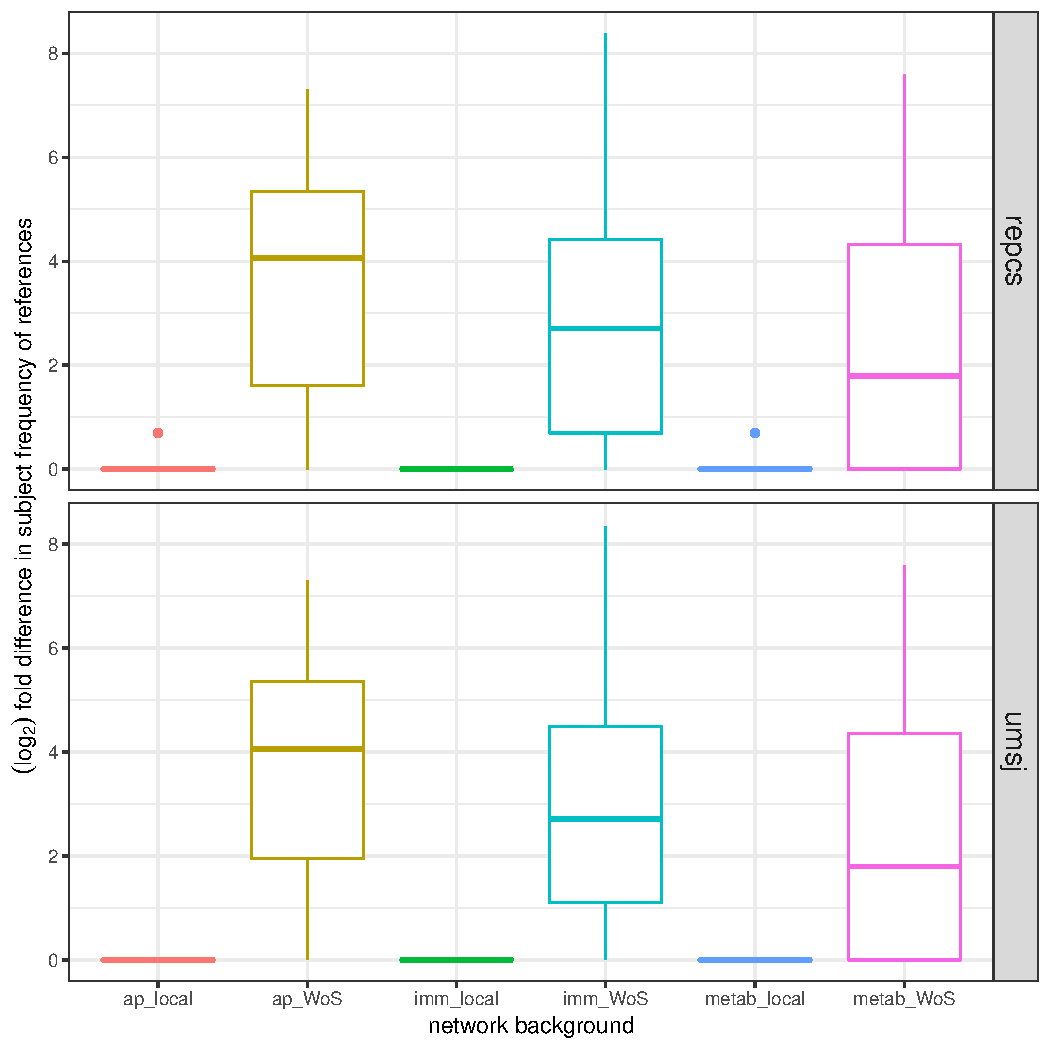
\includegraphics[width=0.6\linewidth]{background-effect}     
\caption{Citation shuffling using the local network preserves the disciplinary composition of references within networks, but using the global network does not.  Publications of type Article belonging to the three disciplinary networks (ap=applied physics, imm=immunology, and  metab=metabolism) were subject to a single shuffle of all their cited references using either the local network (i.e., the cited references in these networks, denoted  bg\_local) or the global network (i.e., references from all articles in WoS, denoted bg\_WoS) as the source of allowed substitutions, where ``bg" indicates the disciplinary network. Citation shuffling was performed using either our algorithm (\emph{repcs}, top row)
 or that of Uzzi et al.~(\emph{umsj}, bottom row).
 The disciplinary composition of cited references before and after shuffling was measured as frequencies for each of 153 sub-disciplines (from the extended subject classification in WoS) and expressed as a fold difference between citation counts grouped by subject for original (o) and shuffled (s) references using the formula (fold\_difference = $ifelse(o > s, o/s, s/o)$) and rounded to the nearest integer. A fold difference of $1$ indicates that citation shuffling did not alter disciplinary composition. Data are shown for articles published in 1985. All eight boxplots are generated from 153 observations each. Null values were set to $1$. Note y-axis: $log_2$ scale.} 
\label{fig:be}
\end{figure}

We also analyzed disciplinary composition at a deeper level using all 153 Subjects in the WoS extended classification and examining the consequences of  citation shuffling within a disciplinary set or all of the Web of Science.  References in publications belonging to these three datasets were summarized as a frequency distribution 153 WoS Subjects as classes. A single shuffle of the references in these datasets or all the references in the corresponding WoS year slice was performed, using either the \emph{repcs}  or \emph{umsj} algorithms, after which subject frequencies were computed again. The fold change in subject frequencies of references before and after shuffling was calculated for these groups using all 153 subject categories and are summarized as boxplots in Fig \ref{fig:be}. As an example, the applied physics dataset contained one reference labeled Genetics and Heredity, but after the shuffle (using the WoS background), acquired 1496 references labeled Genetics and Heredity. Similarly,  the metabolism dataset  contained one reference labeled Philosophy, but after a single shuffle (again using the WoS background) it had 661 occurrences with this label. The data show convincingly that the disciplinary composition of references in a network is preserved when citation shuffling is constrained to the network, but is significantly distorted when the WoS superset is used as a source of substitution. A second inference is that the two algorithms, \emph{repcs} and \emph{umsj}, have equivalent effects in this experiment (and so are only distinguishable for running time considerations).

\begin{table}[ht]
\caption{Model misspecification is reduced by constraining substitutions to the local  disciplinary networks. 
We computed 
Kullback-Leibler (K-L) divergences
between empirical and simulated journal pair frequencies using two different
background networks (local versus global) for each disciplinary network  (applied physics, immunology, and metabolism)
for the years 1985, 1995, and 2005.
% for the three disciplinary datasets (applied physics, immunology, and metabolism) using either the disciplinary network as background or the WoS superset (all\_wos) to generate the null model (Background). 
K-L divergence was calculated using the R seewave package \citep{seewave2008}.  
For every disciplinary network, there is a smaller K-L divergence between simulated and observed data
when using the local network (i.e., the disciplinary network) as compared to the global network (all of WoS). 
Put differently, 
model misspecification is reduced in the constrained model compared to the unconstrained model.
%by  restricting the reference substitutions to the disciplinary network  as compared to treating all substitutions within WoS as equiprobable.
}
\label{tab:kld}
\centering
\begin{tabular}{| ccccc |} 
  \hline
 Disciplinary Network & Year & Background Network & K-L Divergence & Ratio \\ 
  \hline
Applied Physics & 1985 & local & 1.21 &  \\ 
  & 1985 & global & 2.37 & 1.96 \\ 
  & 1995 & local & 0.86 &  \\ 
  & 1995 & global  & 2.37 & 2.77 \\ 
  & 2005 & local & 0.95 &  \\ 
  & 2005 & global  & 2.35 & 2.47 \\ 
    \hline
Immunology & 1985 & local & 0.75 &  \\ 
  & 1985 & global  & 1.68 & 2.24 \\ 
   & 1995 & local & 0.78 &  \\ 
   & 1995 & global  & 1.70 & 2.19 \\ 
   & 2005 & local & 0.73 &  \\ 
  & 2005 & global  & 1.92 & 2.63 \\ 
    \hline
Metabolism & 1985 & local & 1.11 &  \\ 
   & 1985 & global  & 2.24 & 2.02 \\ 
  & 1995 & local & 1.07 &  \\ 
  & 1995 & global  & 2.33 & 2.17 \\ 
     & 2005 & local & 1.19 &  \\ 
   & 2005 & global  & 2.60 & 2.18 \\ 
   \hline
\end{tabular}
\end{table}

 We then tested the conjecture that model misspecification would be reduced by constraining the substitutions to  disciplinary networks by examining the Kullback-Leibler (K-L) Divergence~\citep{kullback_information_1951} between observed and predicted citation distributions, restricted to  the set of journals in a given disciplinary network.  
The results (Table \ref{tab:kld}) confirm this prediction: simulations under the constrained model 
(where the background network is the local disciplinary network) consistently have a lower K-L divergence compared to simulations under the unconstrained model  (where the background network is all of WoS).  Furthermore, the K-L divergence for  the unconstrained model  is generally twice as large as the K-L divergence for the constrained models, with ratios that range from 1.96 to 2.77,  and are greater than 2.0 in eight out of nine cases. These results clearly demonstrate that constraining reference substitutions to the given local disciplinary network better fits the observed data, and hence reduces model misspecification.

\subsection{Calculation of Novelty and Conventionality using the constrained model}  
\begin{figure*}
\centering
\begin{tabular}{ccc}
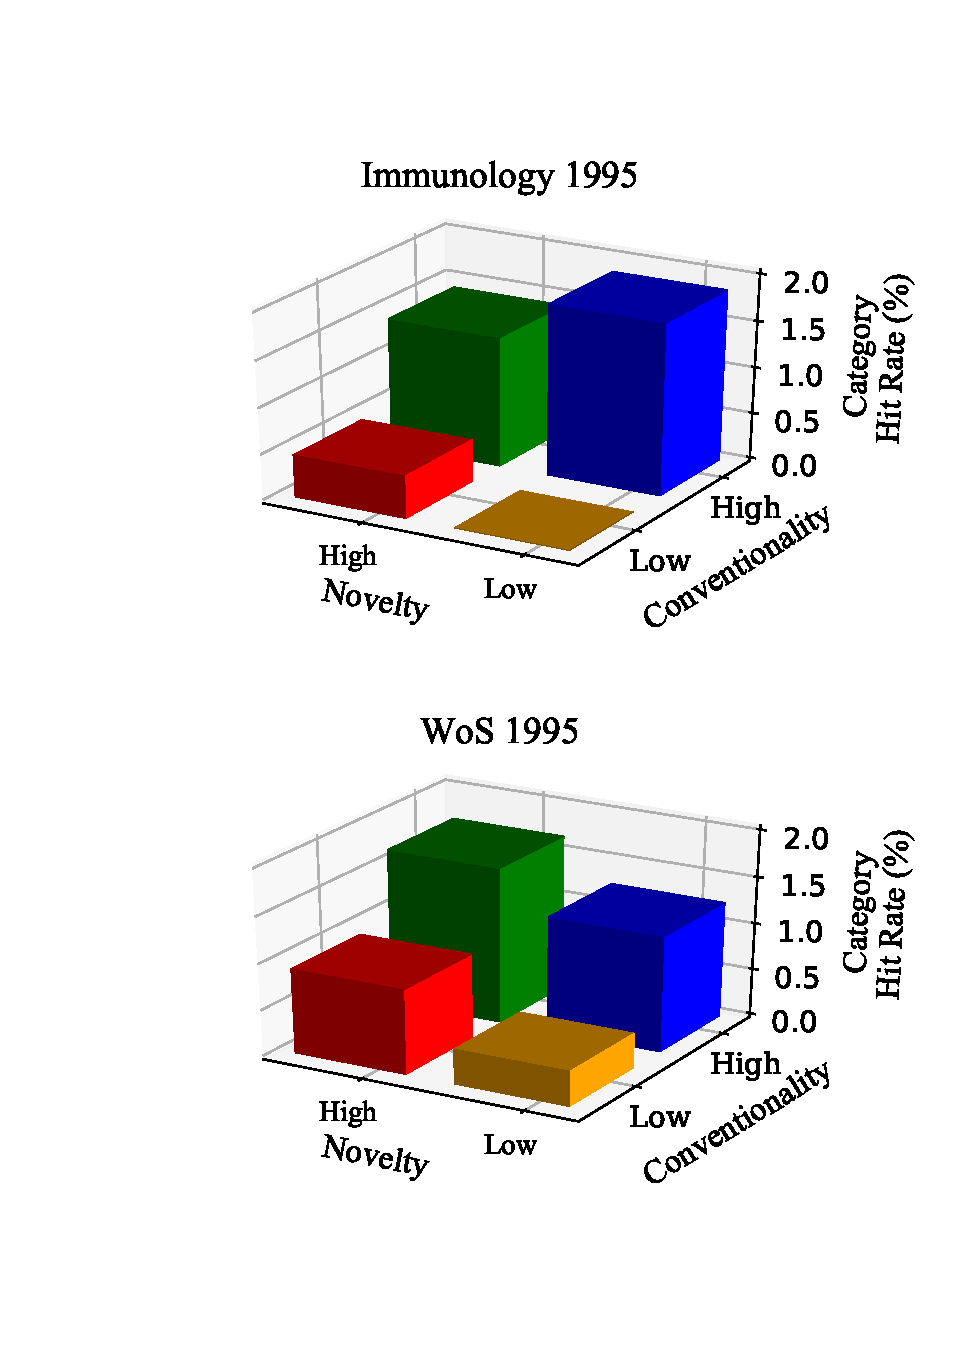
\includegraphics[width=1.5in]{Fig2H01N10.pdf} & 
\includegraphics[width=0.5in]{blank.pdf} & 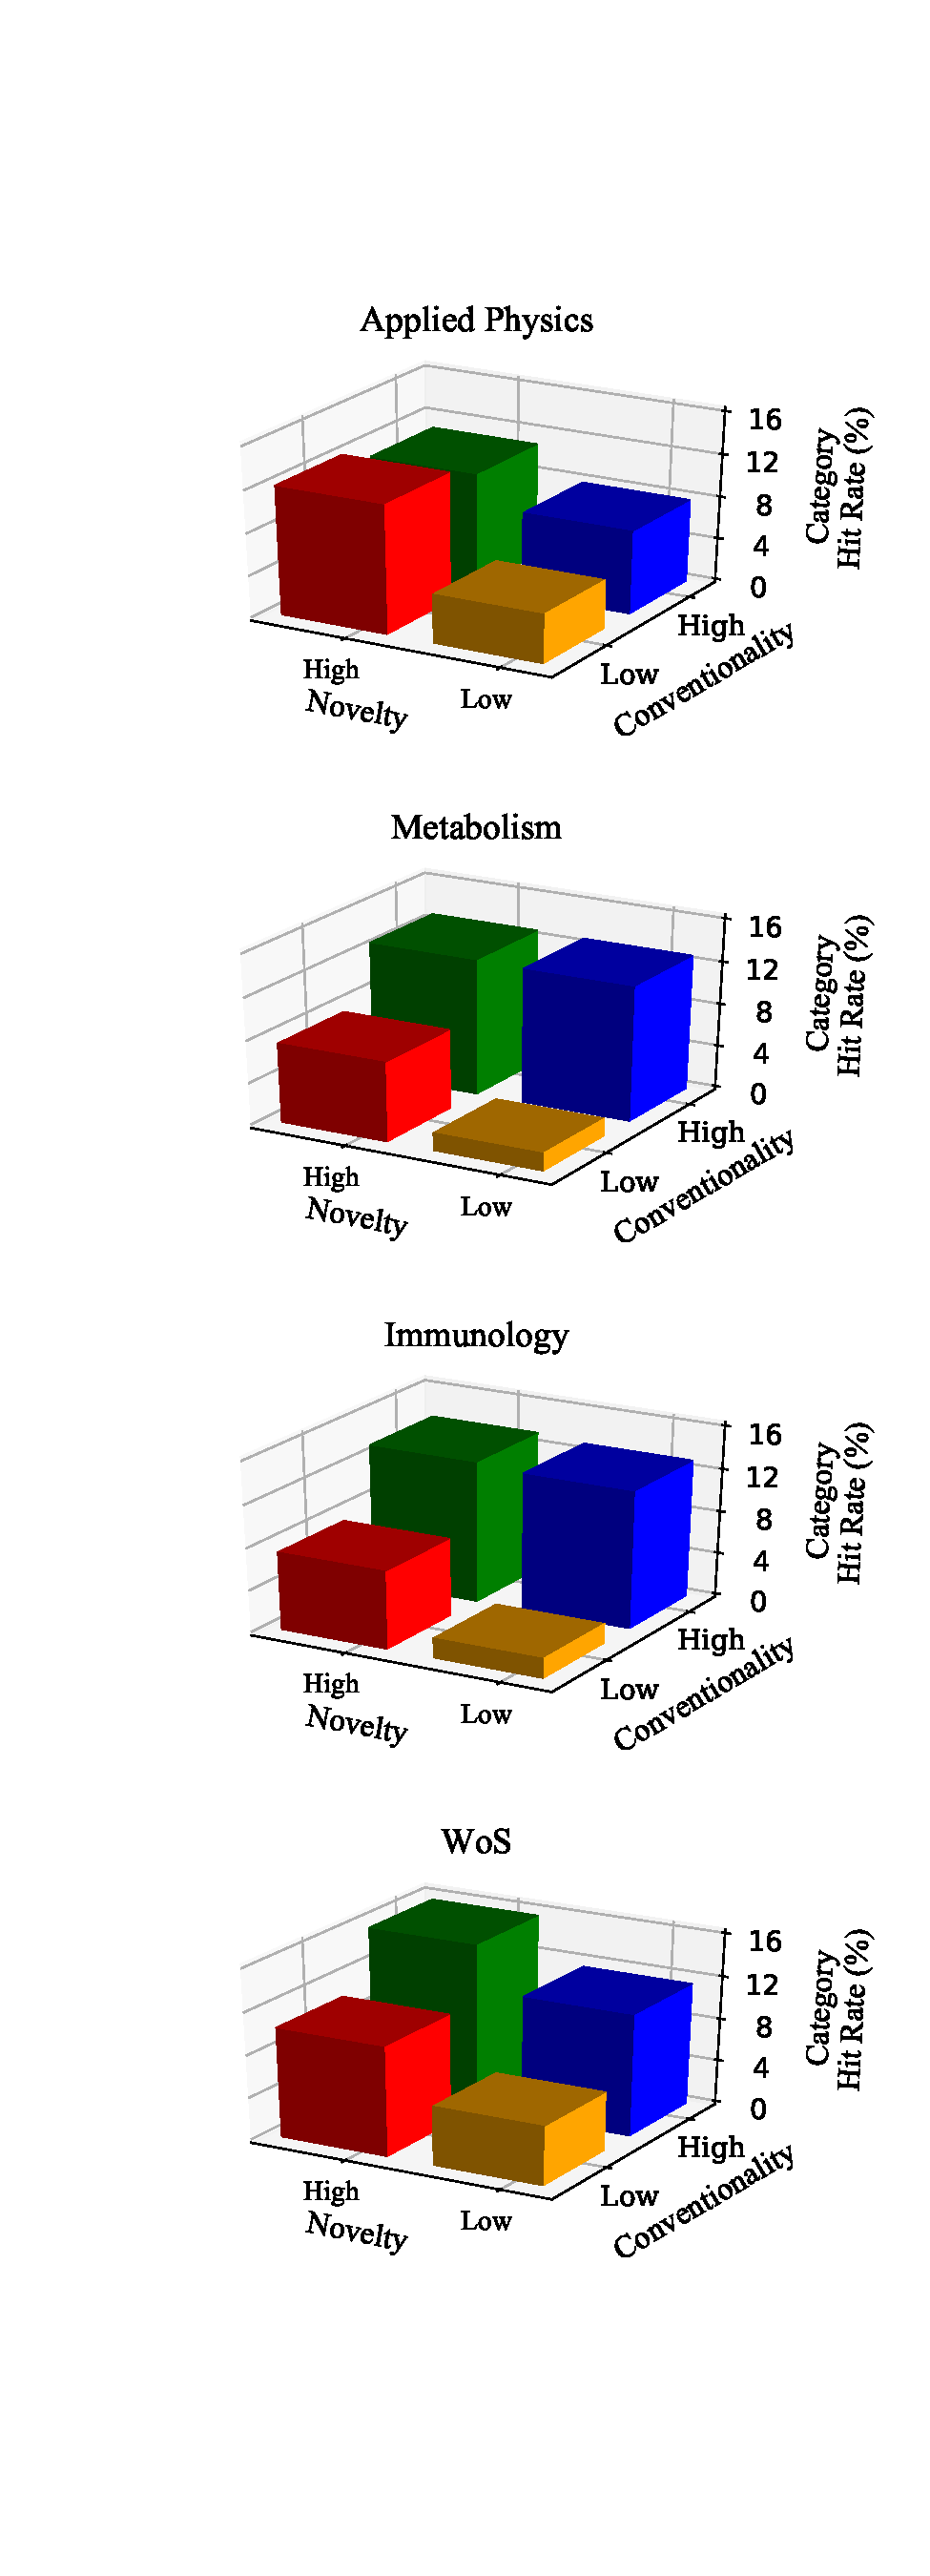
\includegraphics[width=1.5in]{Fig2H10N10.pdf} \\
(a) Top 1\% of cited articles & & (b) Top 10\% of cited articles \\
\end{tabular}
\caption{Effect of using the improved model on  categorical hit rates for Immunology, Applied Physics, and WoS for 1995. Panels (a) and (b) show hit rates for the LNLC, LNHC, HNLC, and HNHC categories for the applied physics, immunology, metabolism, and WoS datasets when hit articles are defined as the top 1\% and top 10\% of articles, respectively.  Novelty in both panels is defined at the 10th percentile of articles' z-score distributions. 
The results for the WoS data set also show that the highest hit rate is for the HNHC category.  Results for the three disciplinary networks all differ from the overall WoS results: the highest hit rates for the immunology and metabolism datasets  are in the LNHC category and the highest hit rate for the applied physics datasets are in the HNLC category.  
\textcolor{blue}{Need numbers for metabolism for the next sentence:} The number of data points in the immunology, applied physics, and WoS data sets are 21,917, 18,305, and 476,288, respectively.  
}
\label{fig:Fig2}
\end{figure*}

Since the constrained model better fits the observed data, we evaluated the distribution of highly cited articles  (i.e., ``hit articles") in the four categories (HCHN, LCHN, HCLN, LCLN), for different thresholds for hit articles. Figure \ref{fig:Fig2}, Panels (a) and (b), compares hit rates for the four categories among the Immunology, Metabolism, Applied Physics, and WoS datasets for 1995, where the hit rate is defined as the number of hit articles in each category divided by the number of articles in the category. 
The calculation for the hit rates for the WoS dataset (bottom row, Figure \ref{fig:Fig2}) mirrors Uzzi et al.'s results, whereby the largest hit rates were for the HNHC category, despite our methodological changes in sampling citations in proportion to their frequency.  However, the trends  for all three  disciplinary networks  are different from those for WoS.Specifically, the highest hit rates for the 1995 immunology and metabolism datasets are in the LNHC category for the top 1\% of cited articles (and tied between LNHC and HNHC for the top 10\%),and the highest hit rates for the 1995 applied physics datasets are in the HNLC category for both the top 1\% and top 10\% of all cited articles.  Thus, the category exhibiting the highest hit rate among highly cited papers depends on the specific disciplinary network and to some extent on the threshold for being highly cited.
 
Furthermore, the categories displaying the greatest hit rate vary  to some extent with the year \textcolor{blue}{(data not shown)}.

We evaluated the statistical significance of the categorical hit rates using multiple methods.  Our first test was based on the null hypotheses that hits were distributed randomly among the four categories with uniform probability in proportion to the number of articles in each category. Rejecting the null hypothesis, using a Chi-Square Goodness of Fit test, supports a non-uniform dispersion of hits with some of the four categories being associated with higher or lower than expected expected hit rates. The null hypothesis was rejected at a $p<0.001$ in all cases in  Figure \ref{fig:Fig2}, with the exception of the immunology and applied physics datasets where hit articles are designated as the top 1\% of articles: valid tests were not possible in those instances due to too few expected hits. The null hypothesis was rejected with $p<0.001$ for all valid tests for all parameter settings, all datasets, and all years: hypotheses tests were valid in 73 of 96 instances. We conclude that it is likely that the distribution of hits among categories is not uniform and that, instead, hit rates vary among the categories in all datasets. 

We also tested the explanatory power of each framework dimension by classifying articles as LN or HN and, separately, as LC or HC. We tested the null hypothesis that hits are distributed between LN and HN (LC and HC) in proportion to the total number of articles assigned to those categories.  That null hypothesis was rejected for the WoS data along both dimensions. Consistent with prior findings, hit articles were overrepresented in the HC category in every instance of WoS data at a $p<0.001$ and also overrepresented in the HN category at a $p<0.001$ in all but two cases: the p-values in those exceptions were $0.002$ and $0.007$.  Hits in the immunology and metabolism data were overrepresented in the HC category with the same statistical significance as for WoS. \textcolor{blue}{The relationship of novelty with hits in the immunology and metabolism data differed dramatically from the WoS, however, with statistically significant findings of hit articles being sometimes overrepresented in the LN category, and sometimes being underrepresented.}  In applied physics, hit articles were positively related with HN with a statistical significance of at least $p<0.10$ in all 12 parameter sets, and at $p<0.05$ in 10 of 12 cases.  Furthermore, a strong positive relationship was found between LC and hit articles in applied physics in 5 of 12 instances with $p<0.10$. These results suggest that (1) both conventionality and novelty are strongly related to hits in the WoS, (2) the conventionality dimension is strongly related with hits in immunology and metabolism and novelty is not, and (3) novelty is more strongly related with hits in applied physics than is conventionality. More generally, we find that the dimensions most strongly related with hit articles vary between disciplinary and broad data sets, and also among disciplines. 

We described concerns with model misspecification along two general dimensions: the background dataset and sampling methodology for the random graph. The differences we found from prior research in terms of which categories demonstrated the highest hit rates were caused both by using disciplinary datasets and our sampling methodology, \textit{repcs},  through the article z-score distributions. 
When z-scores are shifted downward using one algorithm versus another, for example, then the former algorithm can result in an increased percentage of HN articles.
We therefore examined  the extent to which each of our methodological differences contributed to our observations.  
We found that z-scores changed sign more as a consequence of background network (local network or all of WoS) and much less as a consequence of sampling algorithm
 ({\textit{umsj} or \textit{repcs}). 
For example,  on the immunology dataset, 28.6\% of the journal pairs changed signs with our sampling algorithm (\textit{repcs}) as the background network is changed from global (all of WoS) to local, and 
only 2.8\% of z-scores changed signs in the WoS dataset depending on whether 
\textit{umsj} or \textit{repcs} was used. 



We conclude that the choice of background datasets is the source of a majority of differences we observed the categories demonstrating the highest hit rates, although our sampling approach, most notably sampling from a multiset so as to reflect the observed frequencies of individual citations as well as their associated journals and disciplines, can also create material differences.     

\section{Discussion}

The principal difference between the two models is a single parameter--the set of references that can be used as substituents during the substitution process. We provided several lines of evidence that showed that changing this one parameter from to the local disciplinary network reduces model misspecification. Furthermore,  using the constrained model (which allows substitutions only within the local network)  instead of the unconstrained model (which allows substitutions in the entire WoS network) produces different trends in terms of conventionality and novelty, depending on the network. In particular, when using the unconstrained model, highly cited papers were most likely to be
in the HNHC category but this trend does not consistently hold when using the constrained model. Instead, we find that conventionality flavored with novelty is {\em not} generally a feature of impactful research. Further,  high ``novelty" is not always indicative of impactful research (as reflected in citation counts), as shown by both Immunology and Metabolism having their highest hit rates for low novelty (Figure \ref{fig:Fig2}). Of relevance, we found the category displaying the highest hit rate to be sensitive to the study parameters, which include the percentage of articles classified as hits, the z-score percentile threshold that delineates LN and HN, and the publication year. \textcolor{blue}{(data not shown).} 

More generally, these results show that the trends approaching universality in highly cited papers are not robust to changes in thresholds for defining high impact or high novelty articles and may be the consequence of using a random model that has a poor fit to the observed data. On the other hand, while  the constrained model reduces model misspecification compared to the unconstrained model, this does not imply that the constrained model is reasonable nor that trends observed under the constrained model convincingly explain scientific practice. Indeed, there are significant  challenges in using random models to understand human behavior, of which citation practice is one example.

In terms of further work, evaluation in context~\citep{hicks_bibliometrics:_2015} and increased consideration of the disciplinary nature of the scientific enterprise is likely to result in improved models that yield further insight.

\acknowledgments
 We thank the authors of \cite{uzzi_atypical_2013} for sharing their simulation code. We are grateful to Kevin Boyack and Dick Klavans for constructively critical discussions. Research and development reported in this publication was partially supported by Federal funds from the National Institute on Drug Abuse, National Institutes of Health, US Department of Health and Human Services, under Contract Nos. HHSN271201700053C (N43DA-17-1216) and HHSN271201800040C (N44DA-18-1216). The content of this publication is solely the responsibility of the authors and does not necessarily represent the official views of the National Institutes of Health. TW receives funding from the Grainger Foundation. All the code used in this study is freely available from a Github site~\citep{GithubERNIE2019}. Access to the bibliographic data analyzed in this study requires a license from Clarivate Analytics, which had no role in funding, experimental design, review of results, and conclusions presented. 

\authorcontributions 
This study was designed by GC, JB, SD, and TW. Simulations and analysis were performed by AD, DLH, GC, JB, and SD. Infrastructure and workflows used to generate data used in this study were developed by AD, DK, SL, SD, and GC.  All authors reviewed and commented on the manuscript, which was written by GC, JB, and TW.

\bibliography{cocit_r}

\end{document}

\newpage
\section{Residual}
\emph{these remaining sentences require some work}
The varying citation patterns when sampling from a disciplinary-focused dataset versus a broader dataset due, was a cause of journal pair z-scores changing signs in 28.6\% of instances: the effect of any one of these journal pairs on an article's novelty or conventionality is contradictory between broad and, more narrow disciplinary datasets. We contend that the interpretation due to a disciplinary dataset, which preserved citation patterns, is more appropriate and an improvement on current methods. 

\begin{figure}
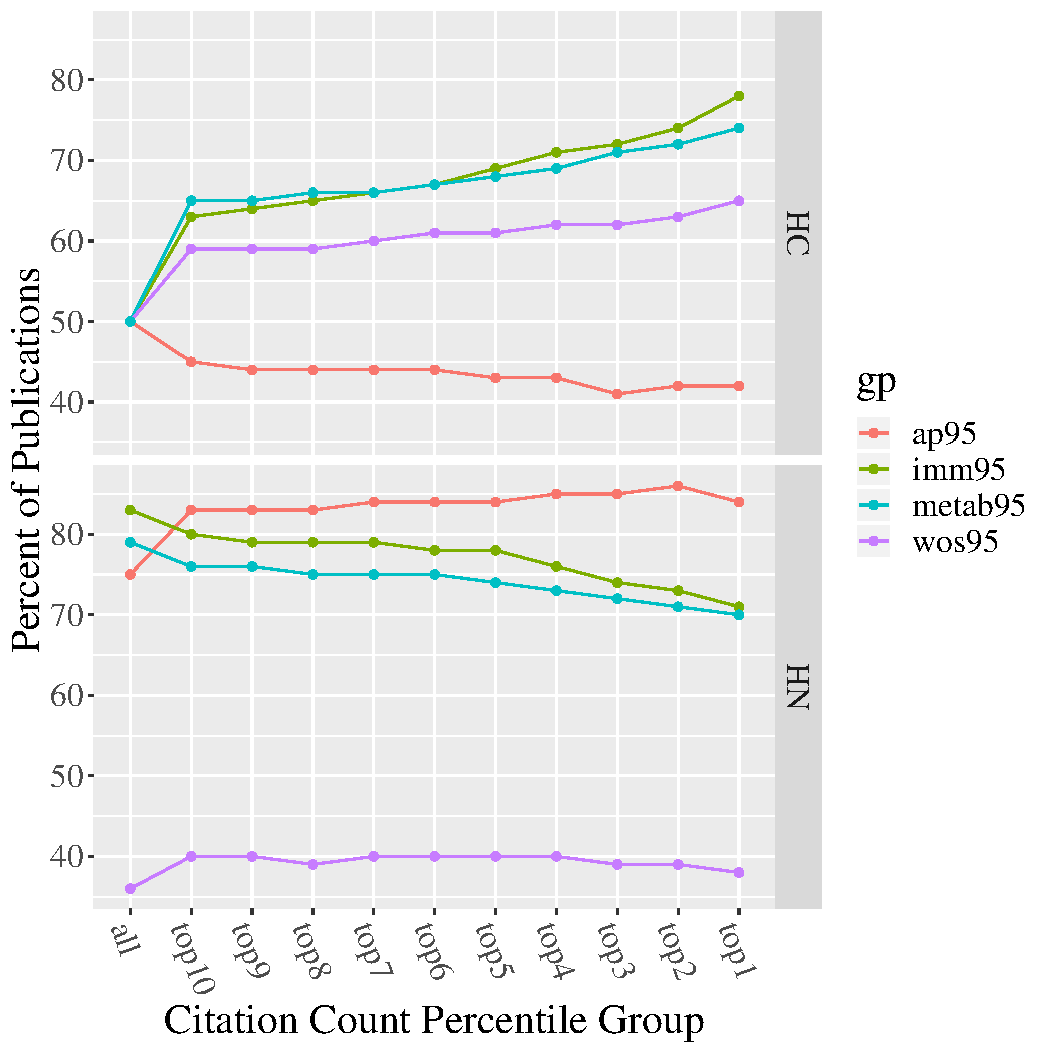
\includegraphics[width=\hsize]{pnas_fig1a}
\caption{Effect of Research Discipline,  Background Network,  and Citation Count on Conventionality and Novelty.
Data are shown for the applied physics (18,305), immunology (21,917), metabolism (97,405) and WoS (476,288) networks for 1995. The number of publications in each network is shown in parentheses. Citation counts shown are cumulative over the first 8 years since publication. 
X-axis: publications were classified into percentile groups based on citation counts (e.g., Top 1 indicates those publications in the top 1\%). Y axis: The percent of applications in each group that are high conventionality (HC) and high novelty (HN). The z-scores are computed for each disciplinary network based on the selected background network; thus, \emph{imm} denotes the immunology network with immunology z-scores and \emph{imm\_wos} denotes the immunology network with z-scores from WoS z-scores. The figure shows striking differences between the WOS network compared to the metabolism and immunology networks: across all networks, the percentage of high conventionality (HC) publications increases with citation counts, while the percentage of high novelty (HN) publications decreases with citation counts for the biological networks but not for WOS.
\label{fig:Fig1}}
\end{figure}

We addressed this consideration by analyzing disciplinary subsets of the scientific literature, thereby restricting random selection of references to only those references in the disciplinary network being studied.
\emph{What about z-scores?} 
We have conjectured that the approach of Uzzi et al. for generating journal-pair z-scores is misspecified in its sampling from a broad dataset and its disregard for the frequency with which journal pairs are citedOur principal consideration was to restrict model misspecification arising from disciplinarily irrelevant references. We addressed this consideration by analyzing disciplinary subsets of the scientific literature, thereby restricting random selection of references to only those references in the disciplinary network being studied.As observed in the Introduction, Monte Carlo simulations that use references from all publications do not account for observed citation practice (sentence needs to be made more eloquent)...

\emph{This paragraph needs work, but I wanted to create a placeholder for the introduction to this subsection.  It uses some of the passages form the former Chacko subsection.} . Like Uzzi et al., we also used a Monte Carlo approach to simulate under a random graph model, although our principal consideration was to restrict model misspecification arising from disciplinarily irrelevant references. We addressed this consideration by analyzing disciplinary subsets of the scientific literature, thereby restricting random selection of references to only those references in the disciplinary network being studied.  In this subsection we demonstrate the effects of model misspecification or Uzzi et al.'s approach and the effectiveness of using disciplinary datasets in resolving the concomitant issues with the former.

Note also in Figure \ref{fig:scatter} that many z-scores values are significantly different between the WoS and Immunology datasets, although the density of points near the origin in Figure \ref{fig:scatter} indicates that some journal pairs change signs between the datasets while their magnitudes are not significantly different. While no metric is without downside, this observation points to a weakness of measuring novelty based simply on the sign of z-scores where no distinction is made between a small negative value and a large negative value, but a negative value of small magnitude is viewed as being significantly different than a small positive value.

We used the criteria of Uzzi to calculate normalized journal pair frequencies (z-scores) and classify publications according to conventionality and novelty. We observe that z-score calculations are sensitive to the background network (disciplinary or WoS). Figure \ref{fig:scatter} shows that the z-scores for the same journal pair can be positive (negative) when computed with respect to one data set but be negative (positive) for another data set. The journal-pair z-scores in Figure \ref{fig:scatter} have consistent signs for both Immunology and WoS data sets in 71.4\% of the instances and different signs for 28.6\% of the journal pairs. When a journal-pair z-score is negative with respect to one dataset and positive with respect to another dataset, articles citing that pair are more likely to be deemed novel in the first instance and less likely to be deemed novel in the second instance.  It seems that any journal pair should either be indicative of novelty or not, but it should never have contradictory implications that depend on the reference dataset. We view, therefore, these contradictions as symptomatic of inappropriately sampling from a broad dataset and ignoring observed citation patterns.  Figure \ref{fig:scatter} reflects that the WoS data set has approximately 44,000 fewer negative z-scores than does the immunology data set, which contributes to its significantly lower percentage of high-novelty articles.  \emph{The plots I made of the cumulative z-score distributions for Immunology and WoS also could be used to demonstrate this phenomenon, although the scatter plot does this more clearly, and it is more striking.  The scatter plot also encodes more data, that is, the matched z-scores for each journal pair.}

\begin{figure}%[tbhp]
\centering
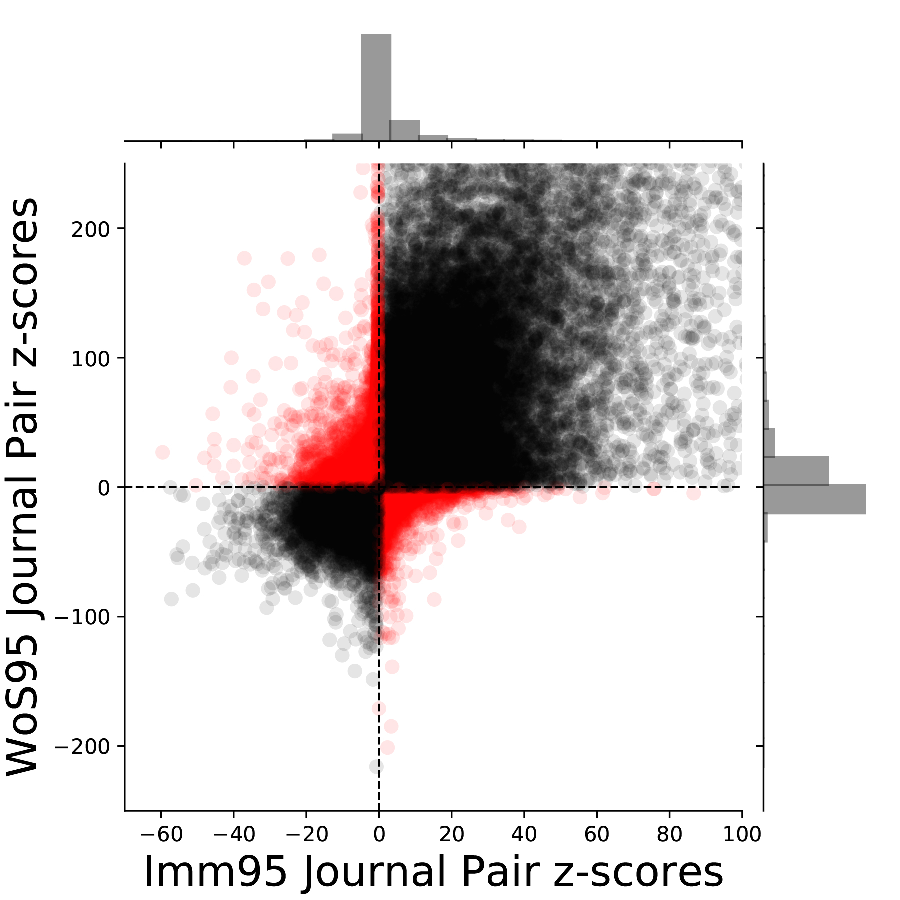
\includegraphics[width=3in]{fig2_scatter_z_scores_flattened.pdf}     %width=.8\linewidth
\caption{Journal pair z-scores vary with background network. 
Scatter plot points (319,005) indicate journal pair z-scores for the 1995 Immunology dataset with two different background networks: the x-axis is based on the local network (1995 Immunology) and the y-axis is based on the entire Web of Science network. Black indicates journal pairs whose z-scores have the same sign when computed for both background networks, while red points indicate the 28.6\% of journal pairs whose z-scores change sign across networks. Regions with deeper hues indicate higher point densities. } %and the histograms show the marginal distributions for each dataset separately.}
\label{fig:scatter}
\end{figure}

%\begin{figure*}
%\begin{tabular}{ccc}
%\includegraphics[width=2.1in]{SIDoc/figs/scatter_z_scores_metab85_WoS_ZoomIn.pdf} & 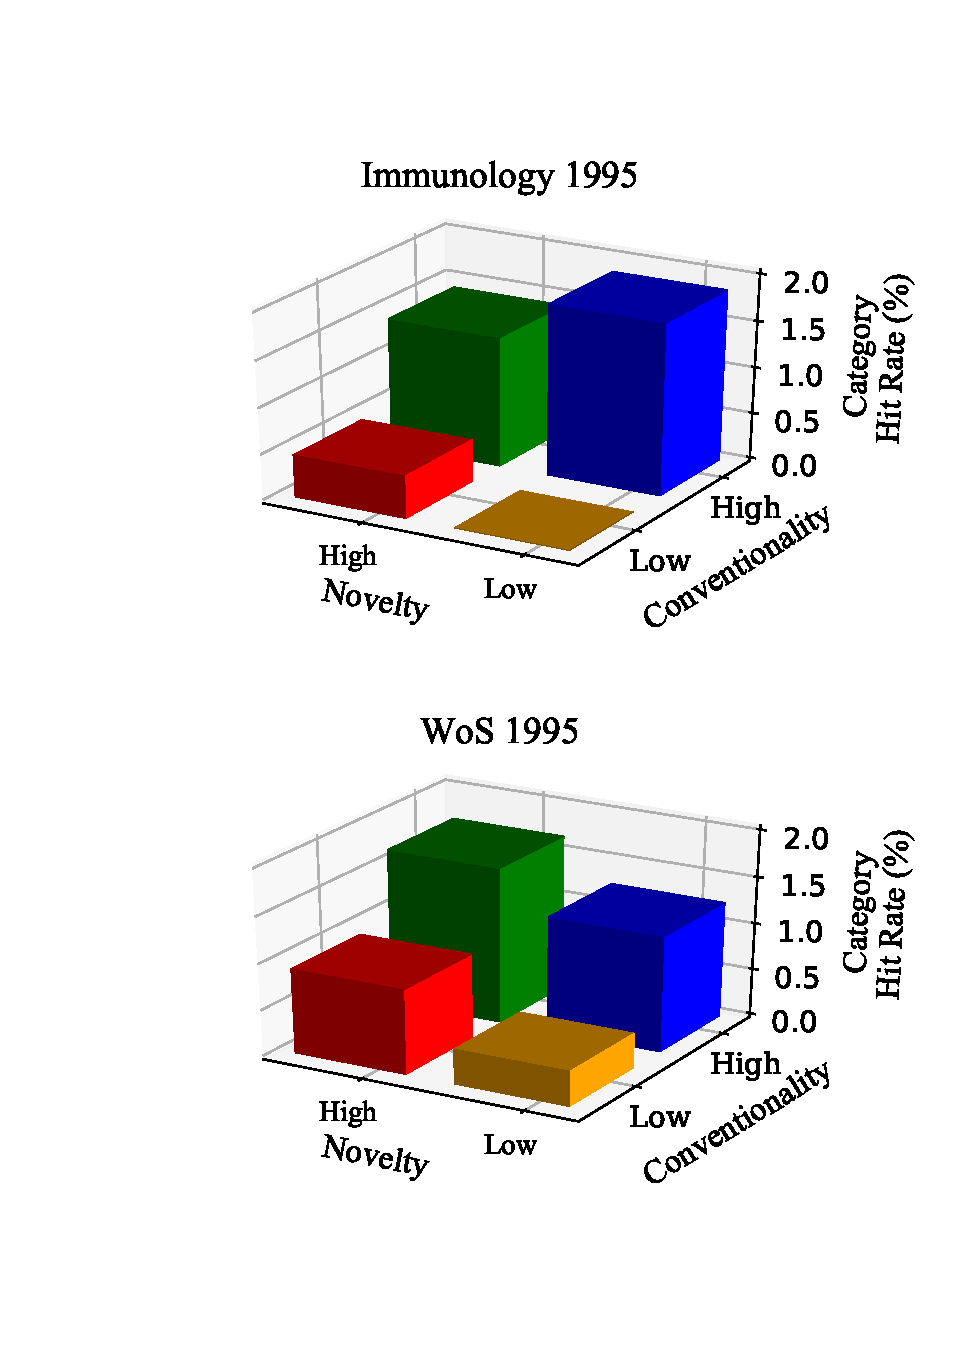
\includegraphics[width=2.1in]{Fig2H01N10.pdf} & 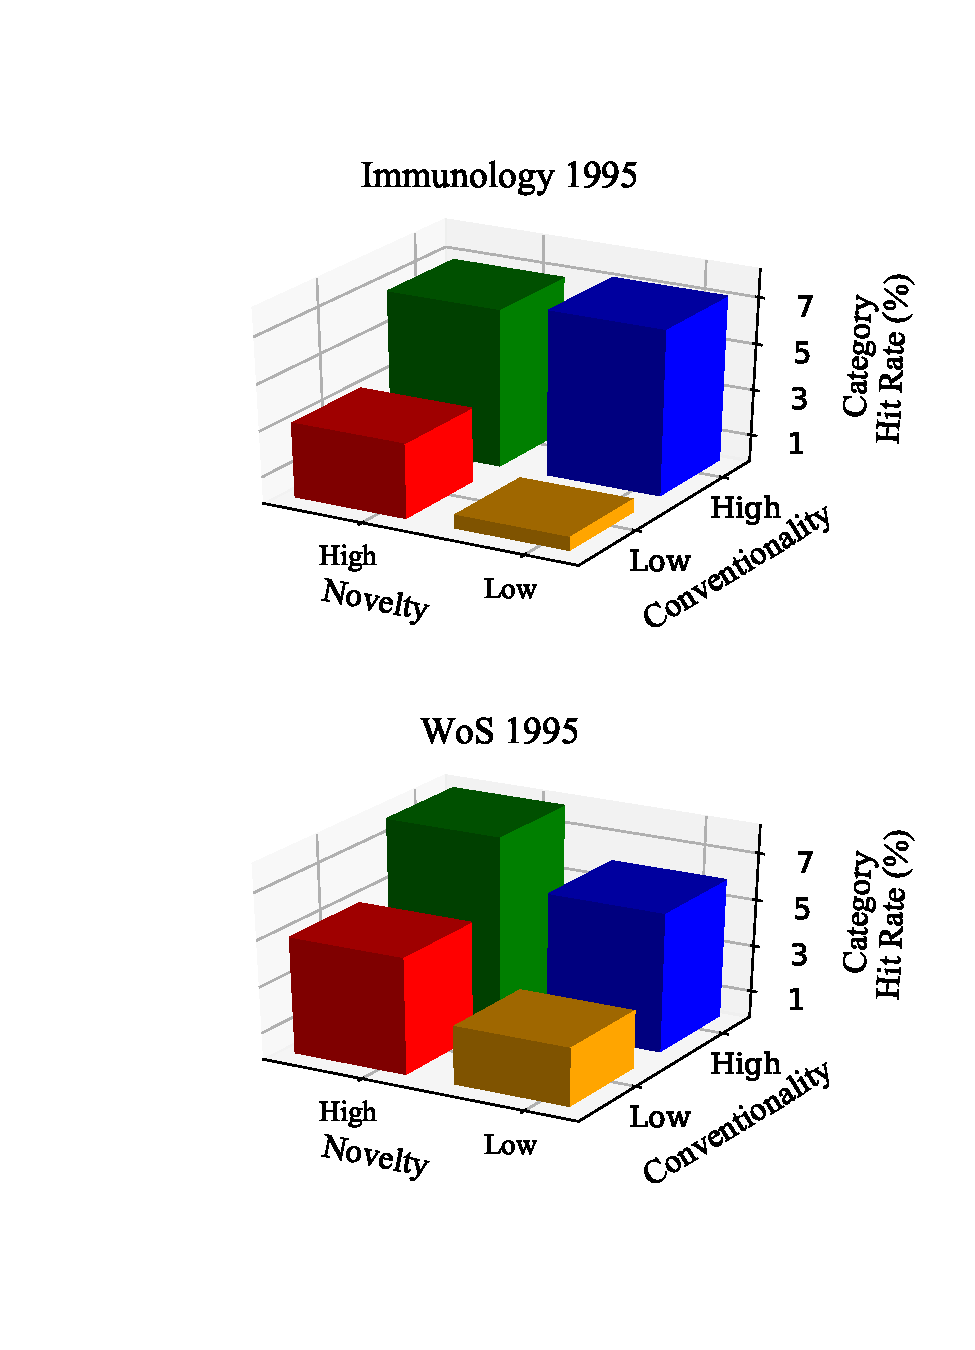
\includegraphics[width=2.1in]{Fig2H05N10.pdf} \\
%(a) & (b) & (c) \\
%\end{tabular}
%\caption{Scatter plot points show journal pair z-scores with respect to the Immunology data set for 1995 on the x-axis and the broad Web of Science on the y-axis. Black indicates journal pairs whose z-scores have the same sign when computed for both data sets while red points indicate journal pairs whose z-scores change sign across data sets. Regions with deeper hues indicate higher point density. The histograms show the marginal distributions of the z-scores for each of the data sets separately.}
%\label{fig:Fig2}
%\end{figure*}

The variation in z-scores with respect to the reference datasets causes the percentages of articles denoted as highly conventional and highly novel to be significantly different, as demonstrated in Figure \ref{fig:Fig1}. \emph{Insert text about Figure \ref{fig:Fig1}.}

\begin{table}%[tbhp]
\centering
\caption[Hit Rates]{Hit Rates by Category for the 1995 datasets. The last four columns indicate the proportion of publications that are hits for each respective category.} \label{Tab:HitRate}
\begin{tabular}{|crrrrrr|}
\hline
& \multicolumn{1}{c}{Hits as \%} & \multicolumn{1}{c}{Novelty}  &  &  &  &  \\ Data Set & \multicolumn{1}{c}{of Articles} & \multicolumn{1}{c}{Percentile} & \multicolumn{1}{c}{LNLC} & \multicolumn{1}{c}{LNHC} & \multicolumn{1}{c}{HNLC} & \multicolumn{1}{c}{HNHC} \\ 
\hline  
Imm95&1\%&10\%& 0.000& 0.019& 0.005& 0.014 \\ 
Imm95&10\%&10\%& 0.017& 0.128& 0.076& 0.129 \\ 
Metab95&1\%&10\%& 0.001& 0.017& 0.006& 0.014 \\ 
Metab95&10\%&10\%& 0.019& 0.130& 0.074& 0.133 \\ 
AP95&1\%&10\%& 0.002& 0.007& 0.012& 0.010 \\ 
AP95&10\%&10\%& 0.047& 0.079& 0.123& 0.109 \\ 
WoS95&1\%&10\%& 0.004& 0.013& 0.009& 0.017 \\ 
WoS95&10\%&10\%& 0.056& 0.115& 0.104& 0.156 \\ \hline

\end{tabular}
\end{table}

%%%%%%%%%%%%%%%%%%%%%%%
%% The bibliography

%\bibliography{cocit_r}

%% No appendices allowed in Network Neuroscience style
%\appendix

\subsection{Sample Subsection}
Text here. Text here. Text here. Text here.
Text here. Text here. Text here. Text here.
Text here. Text here. Text here. Text here.
Text here. Text here. Text here. Text here.

\subsubsection{Sample Subsubsection}
Text here. Text here. Text here. Text here.
Text here. Text here. Text here. Text here.
Text here. Text here. Text here. Text here.
Text here. Text here. Text here. Text here.

\section{Sample equations}
\begin{equation}
\label{eq:rhoCHT}
\rho^{\pi}= \frac{RI + \mathbb{E}_{\pi([L,\tau_L]|\textrm{post})}
\left[C_L(\taupav+\tau_L) \right]   +
\displaystyle{\int_{0}^{P}}{dw~ \mathbb{E}_{\pi_{w_L}}}
\Biggl[\/\sum_{n_{L|[\textrm{pre},w]}}C_L(\tau_L)
\Biggr]            }      {P +
\mathbb{E}_{\pi([L,\tau_L] |\textrm{post})}[\tau_{L}] +\taupav +
\displaystyle{ \int_{0}^{P}}{dw~ \mathbb{E}_{\pi_{w_L}}}   
\Biggl[\sum_{n_{L|[\textrm{pre},w]}}\tau_L\Biggr]  
}
\end{equation}
As long as
$RI - K_LP > 
\frac{1}{\beta}$
\begin{equation}
%\def\theequation{5.1}
\left.\begin{array}{lrcl}
&\rho^{\pi} &=&  \displaystyle\frac{\beta ( RI + K_L \taupav )-1} {\beta
(P+\taupav )}    \\[12pt]
\hbox{and}\hbox to .25in{\hfill}&\mathbb{E}[\tau_L | \text{post}] &=&\displaystyle \frac{P+\taupav}{\beta ( RI -
K_LP)-1}  
\label{eq:analytical_linear}
\end{array}\right\}\hbox to 1.25in{\hfill}
\end{equation} 
Text finishing first page.
Text finishing first page.
Text finishing first page.
Text finishing first page.
Text finishing first page.
Text finishing first page.
Text finishing first page.

\begin{boxedtext}{Comparative Analysis of Different Classes of Networks} 
Going beyond the examination of shared topological features across
nervous systems, the generalized mathematical language of graph theory
also offers tools for the comparison of the organization of brain
networks to other classes of network studied
by different scientific
disciplines. 

Many real-world systems operate as some sort of
interaction or communication network, including, for example, social
networks, gene regulatory networks, computer networks, and
transportation networks. Similar to brain networks, many of these
real-world networks display an efficient small-world organization, a
pronounced community structure with densely connected modules, as well
as the formation of hubs and rich clubs. Going beyond the
comparison of networks within the class of nervous systems, the field
of `comparative network analysis' examines commonalities and
differences across a range of network classes.

\begin{figure}
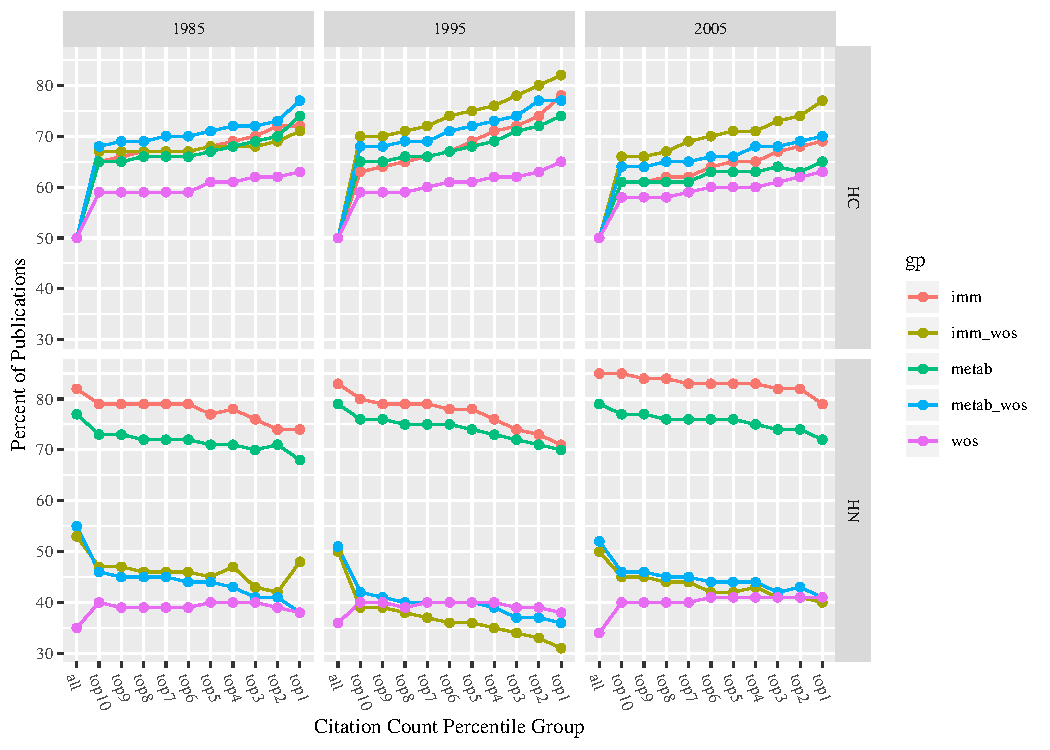
\includegraphics[width=\hsize]{Fig1}
\caption{Here is the caption.}
\end{figure}
\end{boxedtext}

\newpage
\begin{boxedtext}{Comparative Analysis of Different Classes of Networks} 
Going beyond the examination of shared topological features across
nervous systems, the generalized mathematical language of graph theory
also offers tools for the comparison of the organization of brain
networks to other classes of network studied by different scientific
disciplines. Many real-world systems operate as some sort of
interaction or communication network, including, for example, social
networks, gene regulatory networks, computer networks, and
transportation networks. Similar to brain networks, many of these
real-world networks display an efficient small-world organization, a
pronounced community structure with densely connected modules, as well
as the formation of hubs and rich clubs. Going beyond the
comparison of networks within the class of nervous systems, the field
of `comparative network analysis' examines commonalities and
differences across a range of network classes.

\begin{table}[ht]
\caption{Here is the caption.}

\centerline{\begin{tabular}{|c|c|c|}
\hline
one&two&three\\
\hline
four&five&six\\
\hline
\end{tabular}}
\end{table}
\end{boxedtext}

\subsection{Jargon Samples in margin}
One common decision is between working (performing an employer-defined
task) and engaging in leisure (activities pursued for oneself). Working
leads to external rewards such as food and money; whereas leisure is
supposed to be intrinsically beneficial \jargon{Intrinsically beneficial}{The characteristic of
leisure that we enjoy most.} (otherwise one would not want to
engage in it).
%% \jargon has optional argument in square brackets where you can specify
%% the amount of extra space below where it would normally appear when 
%% two \jargon entries are in the same paragraph:
$\beta \in [0,\infty)$\jargon[24pt]{$\beta \in [0,\infty)$}{inverse temperature or degree of
stochasticity-determinism parameter.} is often used to indicate an
important parameter, the stochasticity-determinism parameter.

\subsection{Simple code sample}

\begin{code}
\begin{verbatim}
procedure bubbleSort( A : list of sortable items )
    n = length(A)
    repeat
       newn = 0
       for i = 1 to n-1 inclusive do
          if A[i-1] > A[i] then
             swap(A[i-1], A[i])
             newn = i
          end if
       end for
       n = newn
    until n = 0
end procedure
\end{verbatim}
\end{code}


\subsection{Algorithm environment}
%% \begin{algorithm} takes option [p][b][t][h],  or some combination, like \begin{figure}
%% See documentation for algorithmic.sty for more information on formatting algorithms.

\begin{algorithm}[h]
\caption{A sample in an algorithm environment.}
\begin{algorithmic}
\If {$i\geq maxval$}
    \State $i\gets 0$
\Else
    \If {$i+k\leq maxval$}
        \State $i\gets i+k$
    \EndIf
\EndIf
\end{algorithmic}
\end{algorithm}


\section{Itemized Lists}

\subsection{Roman list:}

\begin{enumerate}
\item[(i)] at high 
payoffs, subjects work almost continuously.
\item[(ii)] at low payoffs, they 
engage in leisure all at once, in long bouts after working.
\item[(iii)] subjects work continuously for the entire price duration, as long as
the price is not very long;
\item[(iv)] the duration of leisure bouts is variable.
\end{enumerate}

\subsection{Numbered list:}

\begin{enumerate}
\item at high 
payoffs, subjects work almost continuously, engaging in little leisure
inbetween work bouts; 
\item at low payoffs, they 
engage in leisure all at once, in long bouts after working, rather
than distributing the same amount of leisure time into multiple short
leisure bouts; 
\item subjects work continuously for the entire price duration, as long as
the price is not very long (as shown by an analysis conducted by
Y-AB, to be published separately);  
\item the duration of leisure bouts is variable.
\end{enumerate}

\subsection{Bulleted list:}

\begin{itemize}
\item at high 
payoffs, subjects work almost continuously, engaging in little leisure
inbetween work bouts; 
\item at low payoffs, they 
engage in leisure all at once, in long bouts after working, rather
than distributing the same amount of leisure time into multiple short
leisure bouts; 
\item subjects work continuously for the entire price duration, as long as
the price is not very long (as shown by an analysis conducted by
Y-AB, to be published separately);  
\item the duration of leisure bouts is variable.
\end{itemize}

\subsection{Description list:}
\begin{description}
\item[High payoffs:] at high 
payoffs, subjects work almost continuously, engaging in little leisure
inbetween work bouts; 
\item[Low payoffs:] at low payoffs, they 
engage in leisure all at once, in long bouts after working, rather
than distributing the same amount of leisure time into multiple short
leisure bouts; 
\item[Continuous work:] subjects work continuously for the entire price duration, as long as
the price is not very long (as shown by an analysis conducted by Y-AB, to be published separately); 
\item[Duration:] the duration of leisure bouts is variable.
\end{description}

\section{Sample figures}

\begin{figure}[h] 
\centerline{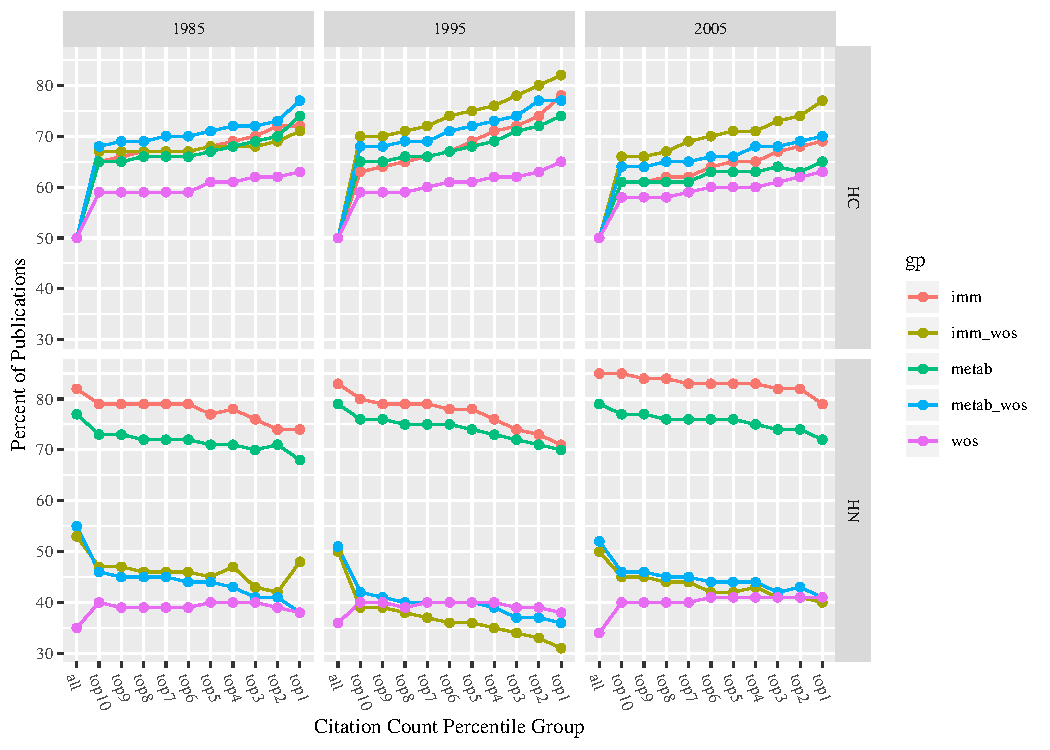
\includegraphics[width=\textwidth]{Fig1.pdf}}
\caption{(Colour online) \textbf{Task and key features of the
 data.} \\
 A) Cumulative handling time (CHT) task. Grey bars denote work
(depressing a lever), white gaps show leisure. The subject must
accumulate work up to a total period of time called the
\emph{price} ($P$) in order to obtain a single reward (black dot) of subjective reward
intensity $RI$. The trial duration is $25\times \mathrm{price}$ (plus
$2$s each time the price is attained, during which the lever is retracted so it cannot
work; not shown).}
\label{fig:task_data}
\end{figure}
%% this command ends a page but does not fill the bottom with white space:
\eject

\begin{figure}[ht] 
\widefigure{\fullpagewidth}{Fig1.pdf}
\caption{(Colour online) \textbf{Task and key features of the
 data.} \\
 A) Cumulative handling time (CHT) task. Grey bars denote work
(depressing a lever), white gaps show leisure. The subject must
accumulate work up to a total period of time called the
\emph{price} ($P$) in order to obtain a single reward (black dot) of subjective reward
intensity $RI$. The trial duration is $25\times \mathrm{price}$ (plus
$2$s each time the price is attained, during which the lever is retracted so it cannot
work; not shown).}
\label{fig:task_data2}
\end{figure}

\newpage
\section{Sample tables}

\begin{table}[!ht]
\caption{Time of the Transition Between Phase 1 and Phase 2$^{a}$}
\label{tab:label}
\centering
\begin{tabular}{lc}
\hline
 Run  & Time (min)  \\
\hline
  $l1$  & 260   \\
  $l2$  & 300   \\
  $l3$  & 340   \\
  $h1$  & 270   \\
  $h2$  & 250   \\
  $h3$  & 380   \\
  $r1$  & 370   \\
  $r2$  & 390   \\
\hline
\multicolumn{2}{l}{$^{a}$Table note text here.}
\end{tabular}
\end{table}

\begin{table}[ht]
\widecaption{Sample table taken from [treu03]\label{tbl-1}}
\begin{widetable}
\advance\tabcolsep-1pt
\small
\begin{tabular}{ccrrccccccccc}
\hline
\bf 
POS &\bf  chip &\multicolumn1c{\bf ID} &\multicolumn1c{\bf X}
&\multicolumn1c{\bf Y} &\bf
RA &\bf DEC &\bf IAU$\pm$ $\delta$ IAU &\bf
IAP1$\pm$ $\delta$ IAP1 &\bf IAP2 $\pm$ $\delta$
IAP2 &\bf star &\bf E &\bf Comment\\
\hline
0 & 2 & 1 & 1370.99 & 57.35\rlap{$^a$}    &   6.651120 &  17.131149 &
21.344$\pm$0.006\rlap{$^b$}  & 2 4.385$\pm$0.016 & 23.528$\pm$0.013 & 0.0 & 9 & -    \\
0 & 2 & 2 & 1476.62 & 8.03     &   6.651480 &  17.129572 & 21.641$\pm$0.005  & 2 3.141$\pm$0.007 & 22.007$\pm$0.004 & 0.0 & 9 & -    \\
0 & 2 & 3 & 1079.62 & 28.92    &   6.652430 &  17.135000 & 23.953$\pm$0.030  & 2 4.890$\pm$0.023 & 24.240$\pm$0.023 & 0.0 & - & -    \\
0 & 2 & 4 & 114.58  & 21.22    &   6.655560 &  17.148020 & 23.801$\pm$0.025  & 2 5.039$\pm$0.026 & 24.112$\pm$0.021 & 0.0 & - & -    \\
0 & 2 & 5 & 46.78   & 19.46    &   6.655800 &  17.148932 & 23.012$\pm$0.012  & 2 3.924$\pm$0.012 & 23.282$\pm$0.011 & 0.0 & - & -    \\
0 & 2 & 6 & 1441.84 & 16.16    &   6.651480 &  17.130072 & 24.393$\pm$0.045  & 2 6.099$\pm$0.062 & 25.119$\pm$0.049 & 0.0 & - & -    \\
0 & 2 & 7 & 205.43  & 3.96     &   6.655520 &  17.146742 & 24.424$\pm$0.032  & 2 5.028$\pm$0.025 & 24.597$\pm$0.027 & 0.0 & - & -    \\
0 & 2 & 8 & 1321.63 & 9.76     &   6.651950 &  17.131672 &
22.189$\pm$0.011  & 2 4.743$\pm$0.021 & 23.298$\pm$0.011 & 0.0 & 4 &
edge \\
\hline\\[-6pt]
\multicolumn{13}{l}{%
Table 2 is published in its entirety in the electronic
edition of the {\it Astrophysical Journal}.}\\[3pt]
\multicolumn{13}{l}{%
$^a$ Sample footnote for table 2.}\\[3pt]
\multicolumn{13}{l}{%
$^b$ Another sample footnote for table 2.}
\end{tabular}
\end{widetable}
\end{table}

\begin{table}[p]
\rotatebox{90}{\vbox{\hsize=\textheight
\caption{Here is a caption for a table that is found in landscape
mode.}
\begin{tabular}{ccrrccccccccc}
\hline
\bf 
POS &\bf  chip &\multicolumn1c{\bf ID} &\multicolumn1c{\bf X}
&\multicolumn1c{\bf Y} &\bf
RA &\bf DEC &\bf IAU$\pm$ $\delta$ IAU &\bf
IAP1$\pm$ $\delta$ IAP1 &\bf IAP2 $\pm$ $\delta$
IAP2 &\bf star &\bf E &\bf Comment\\
\hline
0 & 2 & 1 & 1370.99 & 57.35\rlap{$^a$}    &   6.651120 &  17.131149 &
21.344$\pm$0.006\rlap{$^b$}  & 2 4.385$\pm$0.016 & 23.528$\pm$0.013 & 0.0 & 9 & -    \\
0 & 2 & 2 & 1476.62 & 8.03     &   6.651480 &  17.129572 & 21.641$\pm$0.005  & 2 3.141$\pm$0.007 & 22.007$\pm$0.004 & 0.0 & 9 & -    \\
0 & 2 & 3 & 1079.62 & 28.92    &   6.652430 &  17.135000 & 23.953$\pm$0.030  & 2 4.890$\pm$0.023 & 24.240$\pm$0.023 & 0.0 & - & -    \\
0 & 2 & 4 & 114.58  & 21.22    &   6.655560 &  17.148020 & 23.801$\pm$0.025  & 2 5.039$\pm$0.026 & 24.112$\pm$0.021 & 0.0 & - & -    \\
0 & 2 & 5 & 46.78   & 19.46    &   6.655800 &  17.148932 & 23.012$\pm$0.012  & 2 3.924$\pm$0.012 & 23.282$\pm$0.011 & 0.0 & - & -    \\
0 & 2 & 6 & 1441.84 & 16.16    &   6.651480 &  17.130072 & 24.393$\pm$0.045  & 2 6.099$\pm$0.062 & 25.119$\pm$0.049 & 0.0 & - & -    \\
0 & 2 & 7 & 205.43  & 3.96     &   6.655520 &  17.146742 & 24.424$\pm$0.032  & 2 5.028$\pm$0.025 & 24.597$\pm$0.027 & 0.0 & - & -    \\
0 & 2 & 8 & 1321.63 & 9.76     &   6.651950 &  17.131672 &
22.189$\pm$0.011  & 2 4.743$\pm$0.021 & 23.298$\pm$0.011 & 0.0 & 4 &
edge \\
\hline\\[-6pt]
\multicolumn{13}{l}{%
Table 2 is published in its entirety in the electronic
edition of the {\it Astrophysical Journal}.}\\[3pt]
\multicolumn{13}{l}{%
$^a$ Sample footnote for table 2.}\\[3pt]
\multicolumn{13}{l}{%
$^b$ Another sample footnote for table 2.}
\end{tabular}
}}
\end{table}
\clearpage
\begin{boxedtext}{Tools for comparison of networks} 
Going beyond the examination of shared topological features across
nervous systems, the generalized mathematical language of graph theory
also offers tools for the comparison of the organization of brain
networks to other classes of network studied by different scientific
disciplines. 

From $\mathcal{W}$, we can estimate the variability in the fluctuations of the functional connection between nodes $i$ and $j$ over time as:
\begin{equation}
s_{ij}=\sqrt{\frac{1}{T-L}\sum_{t=1}^{T-L+1}(W_{ij}(t) - m_{ij})}
\end{equation}
where $m_{ij}=\frac{1}{T-L+1}\sum_{t=1}^{T-L+1}W_{ij}(t)$ is the mean
dynamic functional connectivity over time. 

Many real-world systems operate as some sort of
interaction or communication network, including, for example, social
networks, gene regulatory networks, computer networks, and
transportation networks. Similar to brain networks, many of these
real-world networks display an efficient small-world organization, a
pronounced community structure with densely connected modules, as well
as the formation of hubs and rich clubs. Going beyond the
comparison of networks within the class of nervous systems, the field
of `comparative network analysis' examines commonalities and
differences across a range of network classes.
\end{boxedtext}

Example of table continuing over pages:


\begin{center}
\begin{longtable}{ccc@{}}
\caption{ApJ costs from 1991 to 2013
\label{tab:table}} \\[2pt]
\hline
\bf Year & \bf Subscription & \bf Publication \\
 & \bf cost &\bf charges\\
 & \bf(\$) & \bf (\$/page)\\
\hline
\endfirsthead

\multicolumn3c{Table \thetable, \it continued from previous page.}\\[6pt]
\multicolumn3c{ApJ costs from 1991 to 2013}\\[2pt]
\hline
\bf Year & \bf Subscription & \bf Publication \\
 & \bf cost &\bf charges\\
 & \bf(\$) & \bf (\$/page)\\
\hline
\endhead
\\\hline
\\[-8pt]
\multicolumn{3}{r}{\it Table continued on next page}\\ 
\endfoot

\hline
\endlastfoot

1991 & 600 & 100 \\
1992 & 650 & 105 \\
1993 & 550 & 103 \\
1994 & 450 & 110 \\
1995 & 410 & 112 \\
1996 & 400 & 114 \\
1997 & 525 & 115 \\
1998 & 590 & 116 \\
1999 & 575 & 115 \\
2000 & 450 & 103 \\
2001 & 490 &  90 \\
2002 & 500 &  88 \\
2003 & 450 &  90 \\
2004 & 460 &  88 \\
2005 & 440 &  79 \\
2006 & 350 &  77 \\
2007 & 325 &  70 \\
2008 & 320 &  65 \\
2009 & 190 &  68 \\
2010 & 280 &  70 \\
2011 & 275 &  68 \\
2012 & 150 &  56 \\
2013 & 140 &  55 \\
\end{longtable}
\end{center}

\section{Supportive Information}
Here you enter further sources of information, if desired.

%% A possible entry might be:
% No supportive information is available at this time.



